\documentclass[10pt, a4paper,english,spanish]{article}
%\documentclass[10pt,a4paper]{article}
\usepackage[utf8]{inputenc} % para poder usar tildes en archivos UTF-8
\usepackage[spanish]{babel} % para que comandos como \today den el resultado en castellano
\usepackage{caratula}
\usepackage{fullpage} %small margins
\usepackage[parfill]{parskip} %genera saltos entre parrafos
\usepackage[justification=centering]{caption}
\usepackage[usenames,dvipsnames,svgnames,table]{xcolor}
\usepackage{colortbl}
\usepackage[colorlinks=true, linkcolor=black]{hyperref} %Links + Links en el índice
\definecolor{gray}{gray}{0.35}
\definecolor{brightgreen}{rgb}{0.4, 1.0, 0.0}
\definecolor{ReallyLightGrey}{gray}{0.93}
\usepackage{listings}
\usepackage{enumitem}
\usepackage{amsmath} %big brackets
\usepackage[pdftex]{graphicx}
\usepackage[bottom]{footmisc}
\lstset{
    numbers=left,
    breaklines=true,
    tabsize=2,
    basicstyle=\ttfamily\color{gray},
}
\setlength{\parindent}{8pt}
\usepackage{mathtools}
\usepackage[margin=50pt]{geometry}
\usepackage{amsfonts}
\usepackage{flafter}
\usepackage{float}
\usepackage{pdflscape}
\restylefloat{table}
\setcounter{tocdepth}{5}
\setcounter{secnumdepth}{5}

\begin{document}

\materia{Seguridad de la Información}
\submateria{Primer Cuatrimestre de 2017}
\titulo{Trabajo Práctico}
\subtitulo{}

\integrante{Federico De Rocco}{403/13}{fede.183@hotmail.com}
\integrante{Francisco Muchinik}{238/14}{franmuchinik@hotmail.com}
\integrante{Yamil Alis}{742/00}{yamil.alis@gmail.com}
\maketitle
\newpage

\tableofcontents

\section{Logs Seguros}
\section{Logs Seguros}

\subsection{Logs}

Un log es un registro que contiene los eventos ocurridos en un sistema.
Idealmente, todo evento del sistema, en las distintas capas de la arquitectura, se registra en el log.

Con esto, entre otras cosas, se puede auditar el sistema para detectar la existencia de ataques. Por ejemplo, si encontramos en el log del sistema un dump de una base de datos sensible, podríamos estar ante un ataque.
Con esto en cuenta, un atacante tiene motivacíón para intentar borrar sus huellas. Idealmente, éste querría que nadie se entere de que hubo un ataque, porque así los agujeros de seguridad no serán detectados y arreglados, dejando el sistema vulnerable para un futuro ataque. Para esto, debería borrar de los logs únicamente sus acciones. De ser esto imposible, podría intentar simplemente borrar todos los logs. Intentar prevenir esto último, asumiendo un ataque con control completo del sistema, es impráctico, con lo que nos centraremos en proteger los logs de sufrir modificaciones.

\subsection{Protección de Logs}

El Trusted Computing Base (TCB) es el componente responsable de realizar el logging. 
Si se conserva la integridad del mismo, los registros deberián ser seguros. 
Sin embargo, no siempre están libres de bugs que permitan al atacante obtener permisos, o puede ser vulnerado por el atacante solamente porque ya tiene acceso al resto del sistema. Por esto, no conviene asumir que tendremos un TCB seguro.
Hay, sin embargo, opciones de TCB más seguras:

\subsubsection{Imprimirlos}

Una forma clásica de proteger los logs era imprimirlos de forma continua y ordenada. Sin embargo, el sistema que se use para la impresión debe darle prioridad a los logs para que la impresora no se vea sobrecargada.
Un análisis de actividades sospechosas es mucho más difícil.
Se puede comprometer la impresora o las impresiones.

\subsubsection{Write Once Read Multiple (WORM)}
Son discos ópticos de poco ancho de banda de escritura. Dichos discos se extraen una vez que
están llenos. Se puede comprometer la integridad si se sustituyen uno o más discos. Además, es impráctico si el volumen de datos y cantidad de consultas es alto.

\subsubsection{Remote Logging}
Consiste en enviar los registros a otros equipos que los resguarden. Con esta medida el atacante deberá conocer y vulnerar todos estos equipos para poder ocultar el ataque. En este caso, hay que analizar el costo de un servidor externo, y la latencia y disponibilidad, asumiendo que los logs quieren ser consultados frecuentemente. Ademas, como se mencionó, esto no garantiza seguridad necesariamente, dado que el servidor externo podría ser vulnerado también, y vuelve la seguridad de este host un asunto crítico.

Se puede llegar a combinar con replicación local, si se desea tener acceso rápido, para un uso de los logs distinto a auditoría, como puede ser estadísticas de uso.


\subsection{MAC}
Un Message Authentication Code es un mensaje asociado a un otro mensaje original que se envía junto a este último para asegurar su integridad y autenticidad. Dado el original, y una clave necesariamente conocida por ambas partes, se calcula el MAC, y se lo envía con el original, de modo que el recipiente puede, con la clave, regenerar el MAC a partir del mensaje y verificar que coincidan.	Se parte de la hipótesis de que adivinar la clave secreta a partir del mensaje y el MAC no es posible en el corto plazo.

Planteamos entonces que se podría usar MACs para asegurar nuestros logs. Aunque los MACs se usen normalmente en un contexto de una comunicación, podemos pensar los logs como mensajes unilaterales que se leen y verifican mucho después de ser emitidos.

Se calcula un MAC para cada log usando un secreto y se lo loggea junto al mensaje original. Esto permite impedir que, en desconocimiento de ese secreto, el atacante pueda modificar el log.

Sin embargo, en ausencia de un continuo uso de remote logging, este mecanismo
no asegura la integridad de los registros viejos. Esto se debe a que el secreto es usado en el sistema que realiza el logging. 
Si este se compromete, también se obtiene el secreto.


\subsection{Forward Integrity}

Nuestro objetivo es entonces generar un MAC para cada línea de log, que no puedan
ser modificados sin que quede en evidencia ante una auditoría, inclusive si el sistema que genera
los logs es comprometido.
Una entrada del log consiste de un timestamp y el contenido. Como ya se sugirió, un atacante puede intentar comprometer la integridad de los logs para ocultar sus acciones. Podría querer modificar o borrar las entradas relevantes a su ataque.
Para evitar que, inclusive ante el comprosimo del sistema de logging, la integridad de los logs se mantenga, no utilizaremos un único secreto a lo largo del tiempo, sino que iremos actualizando las claves. La idea es que, aunque el atacante posea el secreto en un cierto momento, no podrá obtener ninguno de los secretos anteriores, con lo que no podría modificar correctamente los logs previos a ese momento. Esta propiedad se llama forward integrity.

El algoritmo, sin entrar en detalles, se trata de actualizar los secretos de manera no reversible de forma que el atacante, si compromete el sistema y obtiene el secreto de ese momento, no pueda obtener los anteriores.

La verificación se puede hacer con el secreto inicial, y regenerando programáticamente los siguientes secretos, y asi validando los MACs.

Esto habilita el debate respecto al secreto inicial. Si el secreto inicial es comprometido, el atacante podría modificar los logs arbitrariamente, sin que falle cuando se lo valide. Entonces, el secreto inicial (ni ninguno de los subsiguientes) no debe ser guardado en la memoria del programa de logging, y, en realidad, tampoco debería estar en el sistema, dado que el atacante podría modificarlo o borrarlo. Éste debe estar preferentemente guardado offline, ya que estamos asumiendo un compromiso total del sistema, posiblemente en un medio físico como papel o un disco sin conexión.

Es también importante asegurar que el método de generar los MACs y los secretos sean seguros.

También es importante considerar cada cuanto cambiar el secreto. El período mínimo es de una entrada, que implica generar un nuevo secreto por cada línea. Esto tiene la ventaja de que si el atacante obtiene el secreto, sólo puede afectar las entradas a partir de la más reciente. Si decidimos usar un período mayor, habrá entradas previas que usen el mismo secreto para generar su MAC, que quiere decir que el atacante podrá modificarlas sin problema. Sin embargo, es menos costoso utilizar un período más grande, especialmente si consideramos que los sistemas modernos tienen logs de tamaños considerables.

Para manejar períodos mayores, se pueden introducir ciertas reglas para hacer más seguro el sistema, como puede ser obligatoriamente cambiar el secreto luego de una entrada de log de nivle crítico.


Este sistema deja implícito que debe existir un secreto inicial y si
este se compromete se pierde la seguridad. Por esto el secreto inicial
debe estar guardado en un lugar seguro.
I A la hora de verificar el estado de un registro en particular se debe
calcular su clave en la cadena de hash. Al log guardado se le aplica
la función no reversibles y se calcula el MAC. Si este no coincide con
el almacenado, el registro fue modificado.
I Es igualmente válido utilizar una clave aleatoria para cada entrada en
el registro. Problema: Se deben guardar todas las claves utilizadas.

\section{Servidor Syslog}
\subsection{Servidor syslog con forward integrity}
Para nuestro servidor syslog utilizamos \hyperlink{https://gist.github.com/marcelom/4218010 }{https://gist.github.com/marcelom/4218010} y, sobre este, implementamos nuestro 
mecanismo de logging seguro. Nos basamos en el paper [2] para construir nuestra solución. A continuación, describiremos nuestra implementación.
Generamos un MAC para cada log que no pueda ser modificado sin quedar en evidencia
aunque el sistema que genera los logs sea comprometido. La idea es que el sistema no repita la clave utilizada en los pasos anteriores. Una vez calculado
el MAC se debe descartar dicha clave para evitar que se la pueda obtener. Este proceso se muestra en la siguiente imagen:
\begin{figure}[H]
\centering
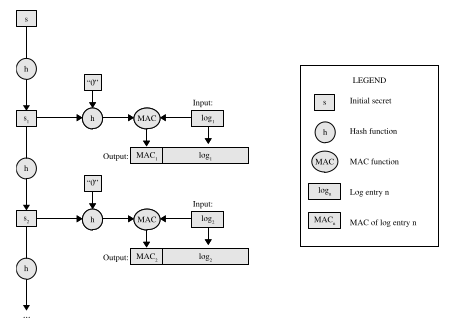
\includegraphics[scale=1]{imagenes/MAC.png}
\end{figure}
Para asegurar la propiedad descripta, generamos la clave actual en base a la inmediatamente anterior como se explica en [1].
Tenemos para el log número i la clave $K_{i}$ que se obtiene aplicándole una función no reversible a
$K_{i-1}$. Una vez calculada $K_{i}$, se borra $K_{i-1}$. Esto último requiere que el FI sea rápido. Si el atacante obtiene control del sistema en el momento que el siguiente log es el número i,
obtendría la clave $K_{i}$. Con la cual no puede regenerar $K_{i-1}$ ni ninguna de las anteriores.
A la hora de verificar el estado de un registro en particular calculamos su clave en la cadena de hash.
Al log guardado le aplicamos la función de hash con la que obtenemos el MAC. Si este no coincide con el almacenado,
el registro fue modificado. La siguiente imagen corresponde al proceso de verificación:
\begin{figure}[H]
\centering
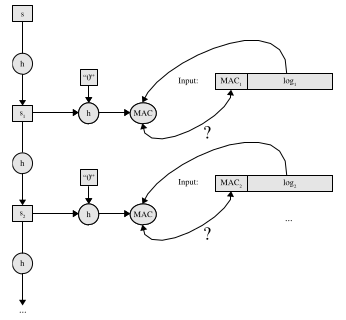
\includegraphics[scale=1]{imagenes/Verification.png}
\end{figure}
Omitimos la posibilidad de utilizar cifrado en los logs.
Nuestra implementación tiene las siguientes particularidades:
\begin{itemize}
\item Utilizamos un secreto inicial, elegido por el administrador del equipo, para iniciar el servidor syslog.
Para cada log que se genere, se calcula su MAC y se guarda.
\item El propio administrador realizara la verificación de los logs aportando el secreto inicial.
\item Los registros de eventos se guardan en un ".log" de solo lectura para un usuario normal.
\item Cada verificación realiza el procedimiento descripto para todos los logs en el registro.
\end{itemize}
\subsection{Alternativas de diseño: Verificación acumulativa}
En lugar de guardar un MAC por cada registro del log, alternativamente se puede guardar solamente uno resultante de un calculo acumulativo. Este mecanismo consiste en que la función de hash toma no solamente la clave, sino también el MAC calculado anteriormente. 
Utilizando esto podemos guardar en un lado el registro de logs y, en otro, el último hash de la cadena. 
Existe un problema en la verificación acumulativa dado que necesita todos los logs previos para comprobar uno. Suponiendo que un atacante modifique el log borrando una parte de él, dejando registros previos y posteriores a la modificación intactos. Tanto el método de verificación que nosotros usamos como su versión acumulativa, podrán detectar el cambio. Además, los dos serán capaces de verificar que los logs previos al ataque están correctos y se puede confiar en ellos. Sin embargo, la verificación acumulativa es incapaz de saber si los registros posteriores están correctos.   
\subsection{Alternativas de diseño: Clave pública}
Una alternativa al uso de la cadena de hash consiste en firmar los logs utilizando una clave privada y verificar la firma con su clave pública. La principal ventaja de esta implementación es que permite que la verificación se pueda realizar con una clave diferente de la que se usa para firmar. 
El proceso consiste en generar un par de claves de los cuales se debe guardar de forma segura la publica(debe asegurar integridad). Utilizando la clave privada se firma una entrada del log que consiste en una secuencia de $n$ claves publicas utilizadas para verificar los $n-1$ siguientes logs. La última clave publica de la secuencia se utilizara para verificar la siguiente entrada que contendrá otra secuencia de claves publicas y así sucesivamente. Cada clave privada usada en la secuencia se descarta inmediatamente. El objetivo es tener las claves publicas a mano para la verificación y, dado que se están firmadas, se puede corroborar su autenticidad. En las siguientes imágenes se muestra el proceso de logging seguro.
\begin{figure}[H]
\centering
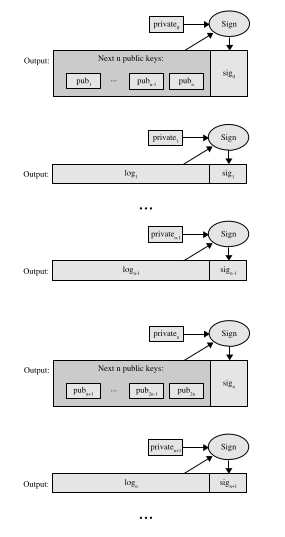
\includegraphics[scale=0.4]{imagenes/PublicKey.png}
\end{figure}
A la hora de verificar, se utilizara la clave publica inicial para el primer log que contiene la cadena de claves publicas. Si es correcto se verificaran cada uno de los siguientes $n$ logs utilizando esta secuencia. Se realizara el proceso para la siguiente entrada utilizando la ultima clave de la cadena y con esto se comprueba la siguiente cadena de claves publicas a utilizar para la verificación. La siguiente imagen ilustra el proceso.
\begin{figure}[H]
\centering
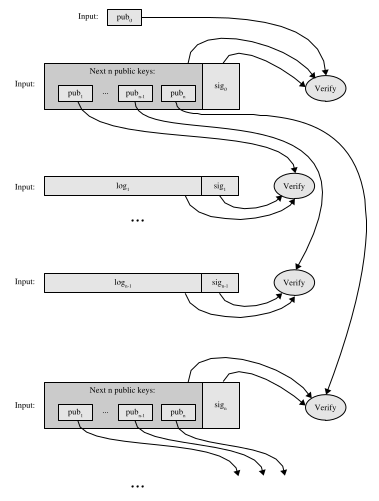
\includegraphics[scale=0.4]{imagenes/PublicKeyVerification.png}
\end{figure}
  
Además de la firma de los logs, se pueden utilizar las claves privadas para cifrar los logs, ocultando la información que contienen.

\section{Bibliografía}
\subsection{Bibliografía}



\begin{thebibliography}{9}
\bibitem{bio1} 
Logcrypt: Forward Security and Public Verification for Secure Audit Logs de Jason E. Holt.
\bibitem{bio2} 
Forward Integrity For Secure Audit Logs de Mihir Bellare y Bennet S. Yee.
\bibitem{bio3} 
Wikipedia. Merkle Tree.
\bibitem{bio4} 
Certificate Transparency RFC 6962.
\bibitem{bio5} 
Mastering Bitcoin. Andreas M. Antonopoulos. Cap\'itulo 7.
\bibitem{bio6} 
$https://gist.github.com/marcelom/4218010$

\end{thebibliography}

\end{document}
